\chapter{Thiết kế hệ thống}
\section{Thiết kế giao diện bằng ứng dụng Figma}
\subsection{Thiết kế giao diện trang hiển thị sản phẩm}
\begin{figure}[H]
    \begin{center}
    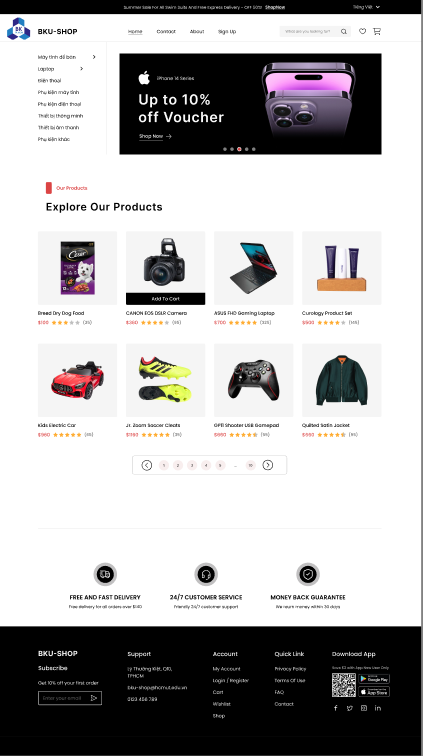
\includegraphics[scale=0.8]{images/hieu/chap-4/display-product-page.png}
    \vspace*{5mm}
    \caption{Thiêt kế giao diện trang hiển thị sản phẩm}
    \end{center}
\end{figure}
\begin{itemize}
    \item \textbf{Phần Header}
    \newline
    Phần đầu trang web gồm các thành phần sau:
    \begin{itemize}
        \item Logo của trang web
        \item Tên trang web
        \item Thanh điều hướng chứa các nút điều hướng đến các trang khác
        \item Ô tìm kiếm sản phẩm
        \item Nút đăng nhập
        \item Giỏ hàng
    \end{itemize}
    \begin{figure}[H]
        \begin{center}
        
\includegraphics[scale=0.5]{images/hieu/chap-4/header.png}
        \vspace*{5mm}
        \caption{Phần đầu trang - Header}
        \end{center}
    \end{figure}

    \item \textbf{Phần Category}
    \newline
    Phần category là một thanh dropdown chứa các danh mục sản phẩm.
    \begin{figure}[H]
        \begin{center}
        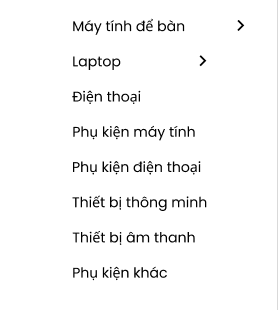
\includegraphics[scale=1]{images/hieu/chap-4/category.png}
        \vspace*{5mm}
        \caption{Phần danh mục sản phẩm - Category}
        \end{center}
    \end{figure}
    \item \textbf{Phần Discount}
    \newline
    Phần discount là một slide chứa các giảm giá của các sản phẩm. Slide sẽ tự chuyển động sau một khoảng thời gian nhất định hoặc có thể chuyển động bằng cách nhấn vào các nút điều hướng.
    \begin{figure}[H]
        \begin{center}
        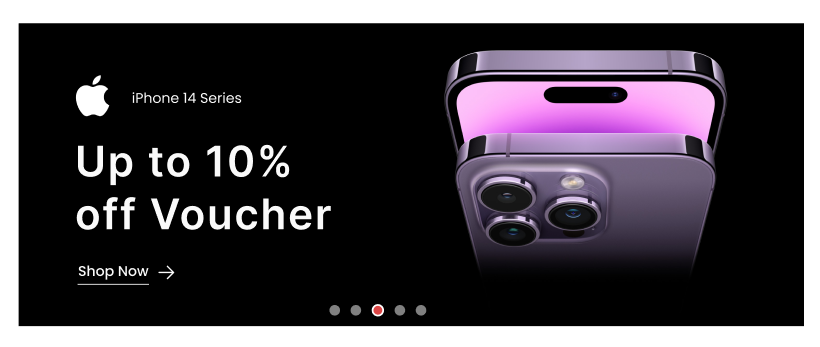
\includegraphics[scale=0.7]{images/hieu/chap-4/discount.png}
        \vspace*{5mm}
        \caption{Phần giảm giá - Discount}
        \end{center}
    \end{figure}
    \item \textbf{Phần Product}
    \newline
    Phần product hiển thị các sản phẩm theo danh mục. Mỗi sản phẩm gồm có:
    \begin{itemize}
        \item Hình ảnh sản phẩm
        \item Tên sản phẩm
        \item Giá sản phẩm
        \item Nút thêm vào giỏ hàng
        \item Nút xem chi tiết sản phẩm
    \end{itemize}
    \begin{figure}[H]
        \begin{center}
        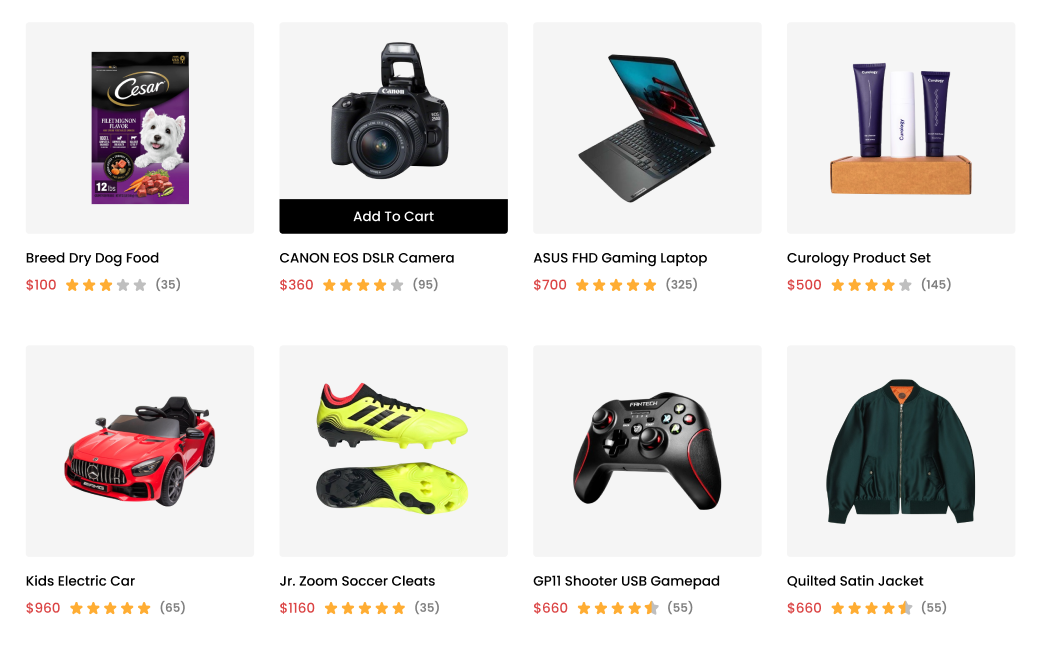
\includegraphics[scale=0.7]{images/hieu/chap-4/product.png}
        \vspace*{5mm}
        \caption{Phần sản phẩm - Product}
        \end{center}
    \end{figure}
    \item \textbf{Phần Footer}
    \newline
    Phần footer là phần cuối trang web chứa các thông tin về trang web, các liên kết đến các trang mạng xã hội, các liên kết đến các trang khác.
    \begin{figure}[H]
        \begin{center}
        
\includegraphics[scale=0.5]{images/hieu/chap-4/footer.png}
        \vspace*{5mm}
        \caption{Phần cuối trang - Footer}
        \end{center}
    \end{figure}
\end{itemize}